\chapter{Aplicación}

\section{Comportamiento de Aplicación}
El punto de vista Comportamiento de la aplicación describe el comportamiento interno de una aplicación; Por ejemplo, ya que realiza uno o más servicios de aplicación. Este punto de vista es útil para diseñar el comportamiento principal de las aplicaciones o para identificar la superposición funcional entre diferentes aplicaciones.
\subsection{Modelo}
\begin{figure}[h!]
	\centering
	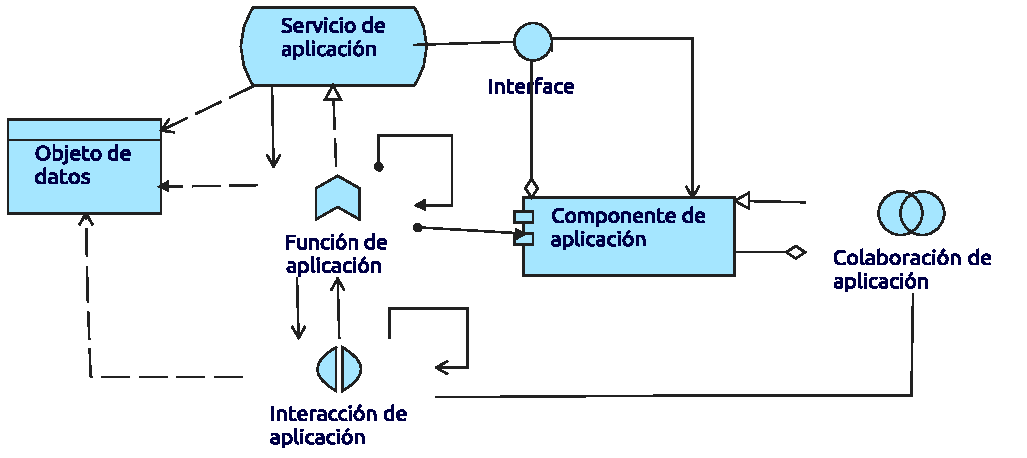
\includegraphics[width=\linewidth]{Arquitectura/Aplicacion/imgs/ComportamientoMetamodelo.pdf}
	\caption{Organización}
\end{figure}
\newpage
\subsection{Caso de Estudio}

\begin{figure}[h!]
	\centering
	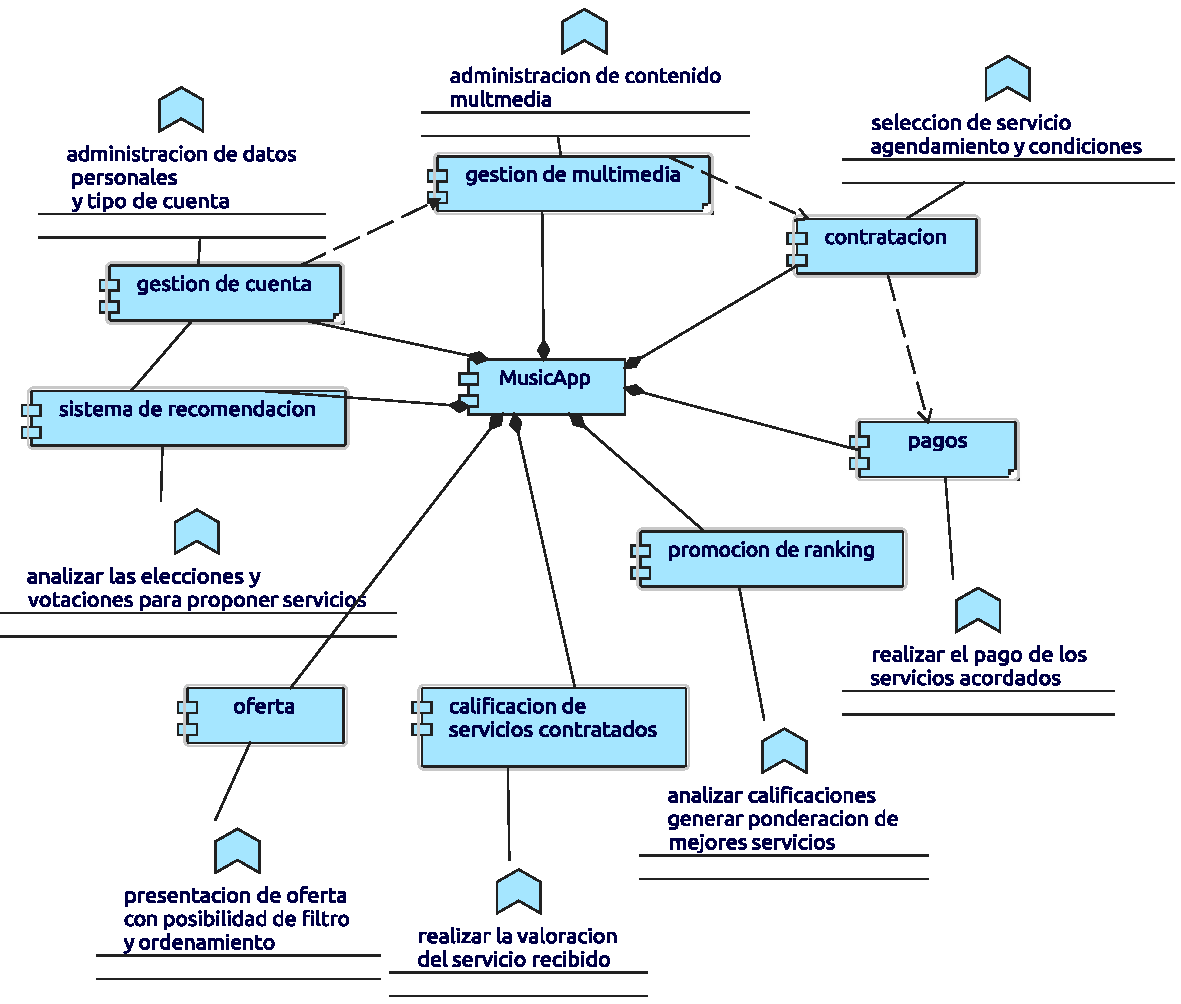
\includegraphics[width=\linewidth]{Arquitectura/Aplicacion/imgs/Comportamiento.pdf}
	\caption{Caso}
\end{figure}

\newpage

\section{Cooperación de Aplicación}
El punto de vista de la Cooperación en la Aplicación describe las relaciones entre los componentes de las aplicaciones en términos de los flujos de información entre ellos, o en términos de los servicios que ofrecen y utilizan. Este punto de vista se suele utilizar para crear una visión general del panorama de aplicaciones de una organización. Este punto de vista también se utiliza para expresar la cooperación (interna) u orquestación de servicios que en conjunto apoyan la ejecución de un proceso de negocios.
\subsection{Modelo}
\begin{figure}[h!]
	\centering
	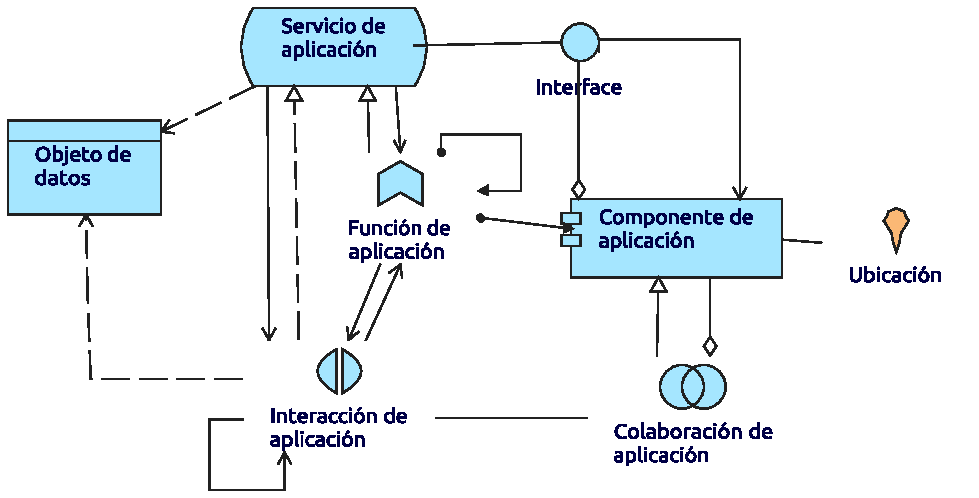
\includegraphics[width=\linewidth]{Arquitectura/Aplicacion/imgs/CooperacionMetamodelo.pdf}
	\caption{Organización}
\end{figure}
\newpage
\subsection{Caso de Estudio}

\begin{figure}[h!]
	\centering
	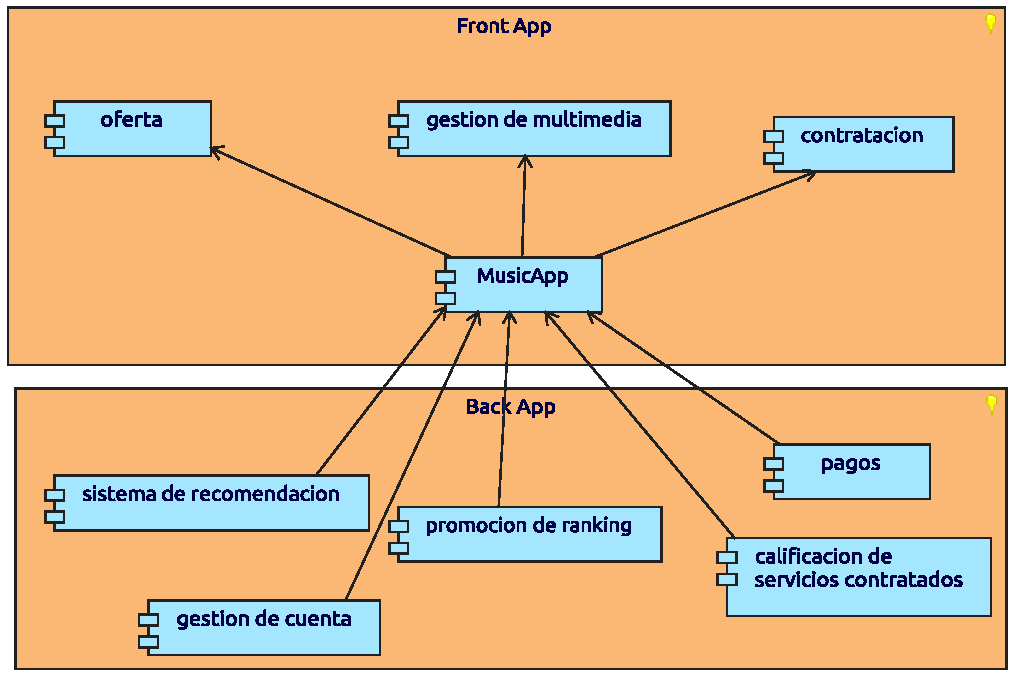
\includegraphics[width=\linewidth]{Arquitectura/Aplicacion/imgs/Cooperacion.pdf}
	\caption{Caso}
\end{figure}

\newpage

\section{Estructura de Aplicación}
El punto de vista de la Estructura de la aplicación muestra la estructura de una o más aplicaciones o componentes. Este punto de vista es útil para diseñar o comprender la estructura principal de las aplicaciones o componentes y los datos asociados; por ejemplo, para desglosar la estructura del sistema en construcción o para identificar componentes de aplicaciones heredadas que sean adecuados para la migración / integración.
\subsection{Modelo}
\begin{figure}[h!]
	\centering
	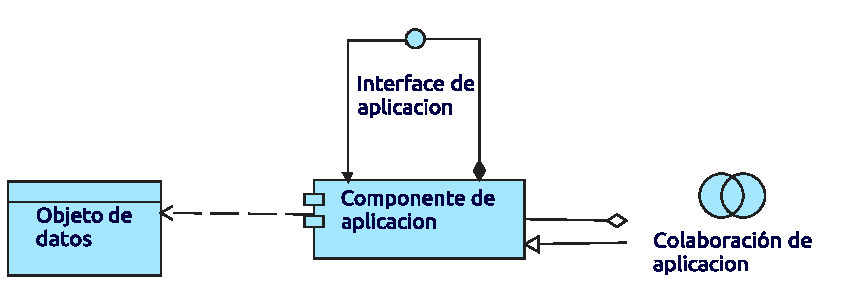
\includegraphics[width=\linewidth]{Arquitectura/Aplicacion/imgs/estructuraMetamodelo.pdf}
	\caption{Organización}
\end{figure}
\newpage
\subsection{Caso de Estudio}

\begin{figure}[h!]
	\centering
	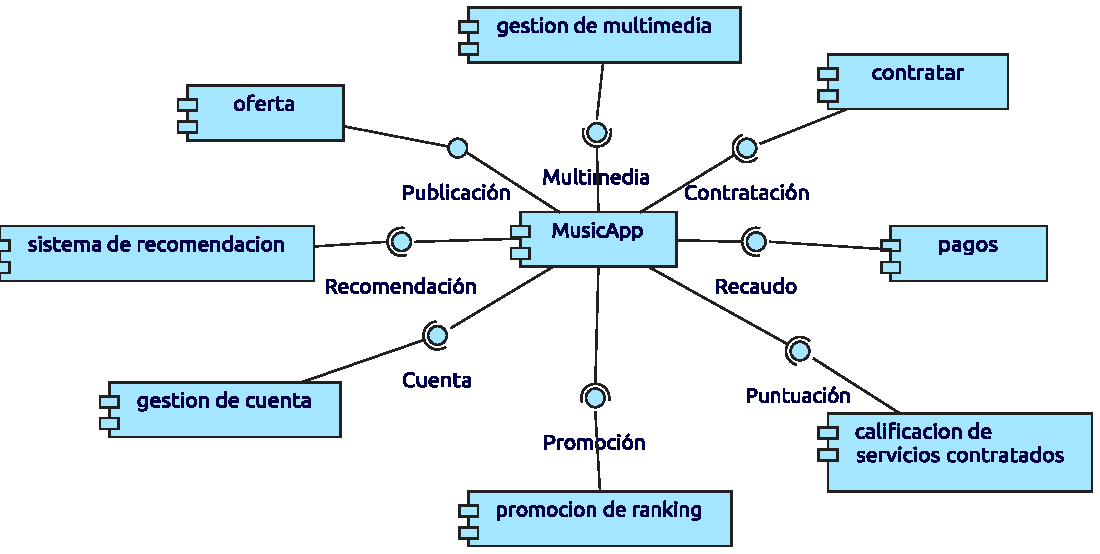
\includegraphics[width=\linewidth]{Arquitectura/Aplicacion/imgs/estructura.pdf}
	\caption{Caso}
\end{figure}


\subsection{Código}

\lstinputlisting[language=Java]{Arquitectura/Aplicacion/fuentes/IContratacion.java}
\lstinputlisting[language=Java]{Arquitectura/Aplicacion/fuentes/ICuenta.java}
\lstinputlisting[language=Java]{Arquitectura/Aplicacion/fuentes/IMultimedia.java}
\lstinputlisting[language=Java]{Arquitectura/Aplicacion/fuentes/IPromocion.java}
\lstinputlisting[language=Java]{Arquitectura/Aplicacion/fuentes/IPublicacion.java}
\lstinputlisting[language=Java]{Arquitectura/Aplicacion/fuentes/IPuntuacion.java}
\lstinputlisting[language=Java]{Arquitectura/Aplicacion/fuentes/IRecaudo.java}
\lstinputlisting[language=Java]{Arquitectura/Aplicacion/fuentes/IRecomendacion.java}
\newpage

\section{Uso de Aplicación}
El punto de vista de Uso de la aplicación describe cómo se usan las aplicaciones para admitir uno o más procesos de negocios, y cómo las usan otras aplicaciones. Se puede usar para diseñar una aplicación identificando los servicios que necesitan los procesos de negocios y otras aplicaciones, o para diseñar procesos de negocios describiendo los servicios disponibles. Además, dado que identifica las dependencias de los procesos de negocios con respecto a las aplicaciones, puede ser útil para los gerentes operativos responsables de estos procesos.
\subsection{Modelo}
\begin{figure}[h!]
	\centering
	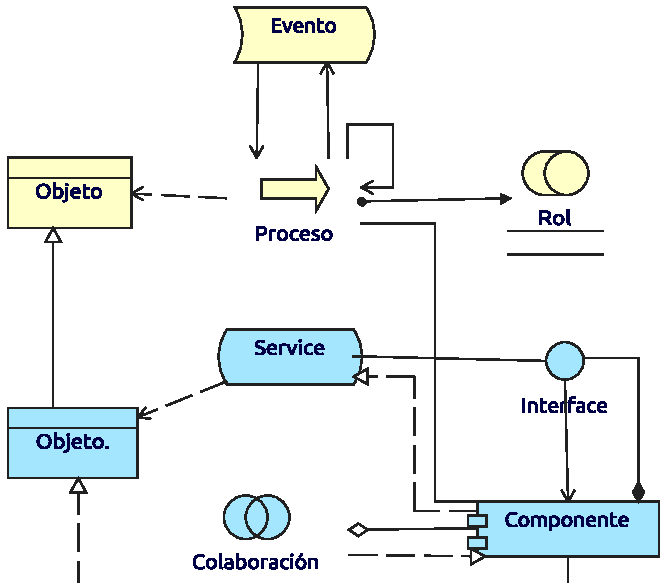
\includegraphics[width=0.9\linewidth]{Arquitectura/Aplicacion/imgs/uso.pdf}
	\caption{Organización}
\end{figure}
\newpage
\subsection{Caso de Estudio}

\begin{figure}[h!]
	\centering
	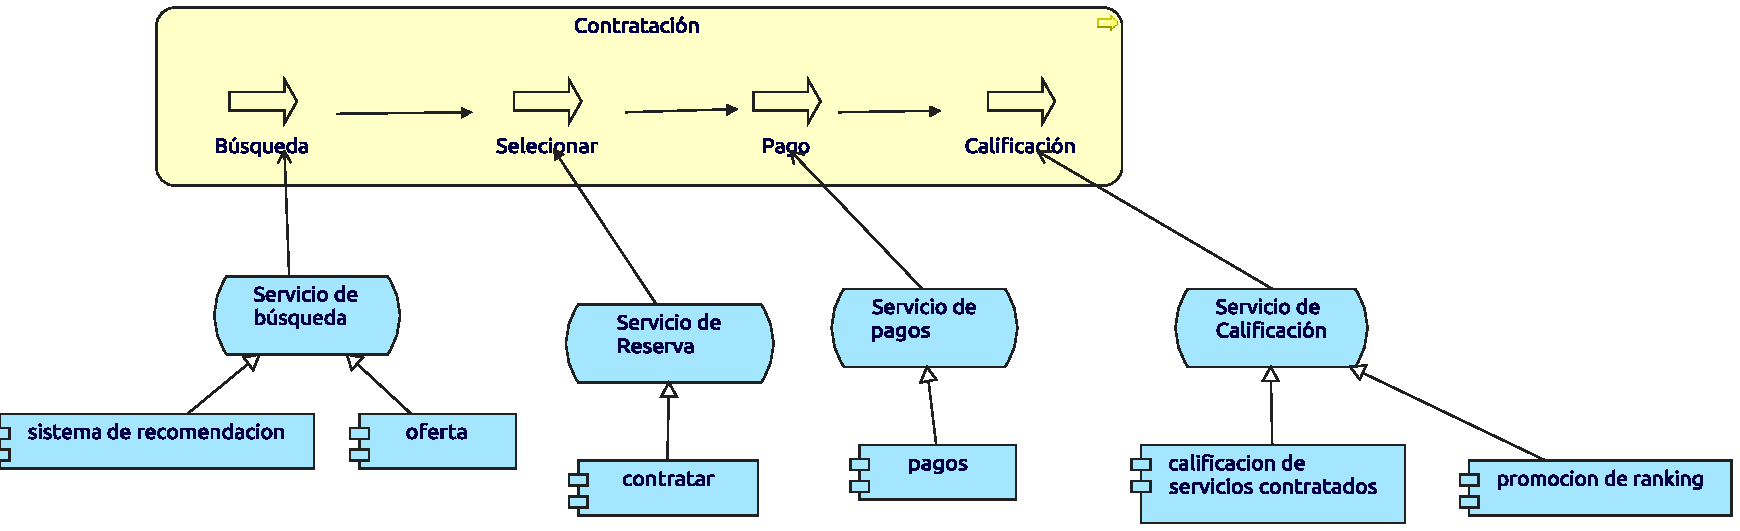
\includegraphics[width=\linewidth]{Arquitectura/Aplicacion/imgs/usoMetamodelo.pdf}
	\caption{Caso}
\end{figure}